
\chapter{SoC Module}
\label{soc_module}

The main purpose of the SoC module is to encapsulate the somewhat complex 
interconnection between the CPU and the Cache/Memory Controller module.

If some project demands that some piece of hardware be directly connected to the
CPU, bypassing the cache, this is where it should be -- an MMU comes to mind.

Any peripherals deemed common enough that they will be present in all projects
might be placed in the SoC module too.

In the current version of the SoC module, there is only one peripheral included 
in it -- a hardwired UART module. There is no penalty for placing peripherals 
ouside the SoC module, so there is no incentive to place them inside. This is 
an implementation option of yours.\\

Bear in mind that, in its current state, the SoC module is little more than a 
vehicle for building demos around the ION CPU. It is not meant as a real-world
SoC, though it might be deloped into one eventually.

\section{SoC Generics}
\label{soc_generics}

    The SoC needs to be configured upon instantiation by setting the following
    generics:

\begin{table}[h]
\caption{SoC module generics\label{tab_soc_generics}}
\begin{tabularx}{\textwidth}{ lll|X }
\toprule
Name & Type & Default value & Description \\
\midrule
\texttt{BOOT\_BRAM\_SIZE}      & integer    & 1024  & Bootstrap BRAM size in 32-bit words. \\
\texttt{OBJ\_CODE}     & t\_obj\_code & (void code) & Bootstrap BRAM contents. \\
\midrule
\texttt{CLOCK\_FREQ}   & integer    & 50e6  & Main clock rate. \\
\texttt{BAUD\_RATE}    & integer    & 19200  & UART baud rate. \\
\midrule
\texttt{SRAM\_ADDR\_SIZE} & integer & 17 & Size of SRAM address bus. \\
\bottomrule
\end{tabularx}
\end{table}   

The current version of the SoC is not very strict in the enforcement of limits 
for the generics. You are advised to use only 'reasonable' values. This will 
be fixed, eventually.

Generic \texttt{CLOCK\_FREQ} is only needed in order to compute the default 
baud period for the internal UART (from the value of generic \texttt{BAUD\_RATE}).


Generic \texttt{BOOT\_BRAM\_SIZE} will determine the size of the internal 
bootstrap BRAM. This generic \emph{can't be zero}; in the current version of
the SoC, the BRAM can't be disabled or omitted.

Note that if the size of the bootstrap BRAM is not enough to hold the whole 
bootstrap code provided in generic \texttt{OBJ\_CODE}, the code \emph{will 
be sineltly truncated!}. Usually this will result in an early crash.

Generic \texttt{OBJ\_CODE} is used at synthesis time to initialize the bootstrap
BRAM. This generic is meant to contain boostrap code, as seen in section 
~\ref{bootstrap_code}). It can be omitted, in which case the bootstrap BRAM
will be initialized to all zeros.


\section{SoC Ports}
\label{soc_ports}

\begin{figure}[h]
\makebox[\textwidth]{\framebox[9cm]{\rule{0pt}{9cm}
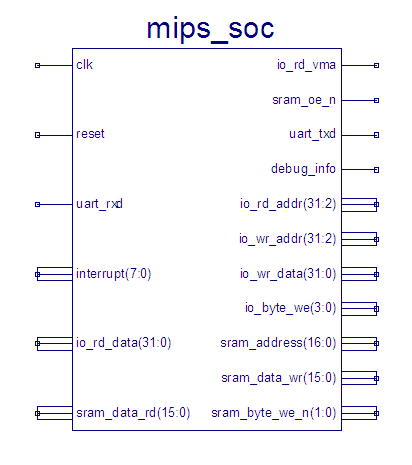
\includegraphics[width=8cm]{img/soc_symbol.png}}}
\caption{SoC module interface\label{soc_symbol}}
\end{figure}

\begin{table}[h]
\caption{SoC module interface ports}
\begin{tabularx}{\textwidth}{ lll|X }
\toprule
Name & Type & Width & Description \\
\midrule
clk                 & in    & 1  & Clock input, active rising edge. \\
reset               & in    & 1  & Synchronous global reset. \\
\midrule
sram\_address       & out   & 16 & Memory word address (bit 0 absent). \\
sram\_data\_wr      & out   & 16 & Memory write data. Only valid when one of the \\
                    &       &    & memory byte write enable outputs is active.\\
sram\_data\_rd      & in    & 16 & Memory read data. Latched when xxx. \\
sram\_byte\_we\_n   & out   & 2  & Memory byte write enable, active low.  \\
                    &       &    & (0) enables the low byte (7 downto 0) \\
                    &       &    & (1) enables the high byte (15 downto 8). \\
\midrule
io\_rd\_addr        & out   & 30 & I/O port read address (bits 1..0 absent). \\
                    &       &    & Only valid when io\_rd\_vma is high. \\
io\_wr\_addr        & out   & 30 & I/O port write address (bits 1..0 absent). \\
io\_wr\_data        & out   & 32 & I/O write data.  Only valid when one of the \\
                    &       &    & i/o byte write enable outputs is active.\\
io\_rd\_data        & in    & 32 & I/O read data. Latched when xxx. \\
io\_byte\_we        & out   & 4  & I/O byte write enable, active high. \\
                    &       &    & (0) enables the low byte (7 downto 0) \\
                    &       &    & (3) enables the high byte (31 downto 24). \\
io\_rd\_vma         & out   & 1  & Active high on i/o read cycles. \\
\midrule
uart\_rxd           & in    & 1  & RxD input to internal UART. \\
uart\_txd           & out   & 1  & TxD output from internal UART. \\
\midrule
interrupt           & in    & 8  & Interrupt request inputs, active high. \\
\bottomrule
\end{tabularx}
\end{table}

As you can see in figure~\ref{soc_symbol} (symbol generated by Xilinx ISE), 
the SoC has the following interfaces:

\begin{enumerate}
    \item Interface to external static asynchronous memory (SRAM, FLASH...).
    \item Interface to on-chip peripherals.
    \item Interrupt inputs.
    \item Debug port.
\end{enumerate}

These interfaces will be explained in the following subsections. The top module
for the demo supplied with the project (c2sb\_demo.vhdl) will be used for 
illustration.

\emph{NOTE}: This section needs a lot of elaboration -- ideally this should be 
equivalent to a datasheet in thoroughness and detail. This work, like many 
other parts of this project, will have to wait.

\subsection{SoC interface to static memory}
\label{soc_if_sram}

The interface to external memory in the SoC module is essentially that of the 
internal cache/memory controller. Its timing is described in section 
~\ref{cache_state_machine}.\\

The SoC inputs are meant to be connected straight to the FPGA i/o pins. The only
trick is the bidirectional memory data bus: as you can see, the SoC data buses 
are unidirectional and thus you will need to provide an interconnection
external to this module. This interconnection shall include the requisite 
3-state buffers:

\begin{verbatim}
sram_databus <= sram_data_wr when sram_byte_we_n/="11" else (others => 'Z');
\end{verbatim}

The top level \emph{c2sb\_demo} module can be used as a fully tested example of 
how to use this interface to connect to a common 16-bit-wide SRAM chip 
(ISSI IS61LV25616).

In reviewing the top module source, note that I had to adapt the dual 
byte-write-enable outputs to the SRAM
configuration of a single write-enable plus dual byte-enable inputs.

Note too that the static memory bus of the SoC module is used to access both the 16-bit wide SRAM 
and an 8-bit wide FLASH. These chips are connected to separate buses on the 
target board, so the top c2sb\_demo module needs to conflate both buses before connecting 
them to the SoC. This is why a multiplexor is used in the \texttt{mpu\_sram\_data\_rd}
bus. A real-world board would probably have the SRAM and the FLASH connected 
to the same bus, simplifying the interface logic.
   
    
\subsection{SoC interface to peripherals}
\label{soc_if_io}

    Every CPU access to an area designated as I/O (see ~\ref{soc_memory_map}, memory map)
    will trigger a read/write cycle on this interface.
    
    I/O ports are synchronous, byte accesible registers meant to be implemented
    within the FPGA. I/O ports do not support wait states.
    
    The I/O interface has separate input and output buses. 
    
    In an output cycle, one or more lines of signal \texttt{io\_byte\_we} will be
    asserted for one clock cycle. Signals \texttt{io\_wr\_addr} and \texttt{io\_wr\_addr} will
    be valid as long as \texttt{io\_byte\_we} is asserted.

    In an input cycle, \texttt{io\_rd\_vma} will be asserted for one cycle and the input
    data should be present at \texttt{io\_rd\_data} at the end of the following clock 
    cycle. The full read operation extends over two clock cycles.
    
\subsection{SoC interrupt inputs}
\label{soc_irqs}
    
    The present version of the CPU does not have support for hardware interrupts 
    and therefore these signals are not used yet and are unconnected. 
    Hardware interrupts will be implemented in some future version as 
    time permits.

\subsection{SoC debug port}
\label{soc_debug_port}
    
    The debug port is a VHDL record (\texttt{t\_debug\_info}, defined in 
    package \emph{mips\_pkg}), which holds some internal CPU status flags that 
    can be useful while debugging the core. It is not meant to be useful for 
    a real application.
    
    Currently the record holds only two flags:
    
    \begin{itemize}
    \item \texttt{cache\_enabled}, asserted when the cache is enabled.
    \item \texttt{unmapped\_access}, asserted when some access to an unmapped 
    address is made.
    \end{itemize}

    The current version of the demo connects these signals to some on-board 
    LEDs. 

    
\section{SoC Memory Map}
\label{soc_memory_map}    
    
    The \emph{memory map} determines the type of memory that is connected to 
    each of a number of predefined address rangess (see section 
    ~\ref{memory_map_definition}).
    It is defined in package \emph{mips\_pkg} and it is implemented in the 
    \emph{mips\_cache} module.
 
\begin{table}[h]
\caption{SoC module memory map\label{tab_soc_memory_map}}
\begin{tabularx}{\textwidth}{ lll|X }
\toprule
Address range & Type & Wait States & Intended usage \\
\midrule
\texttt{0xb8000000-0xbfffffff}   & BRAM    & 0  & SoC internal boot BRAM. \\
\midrule
\texttt{0x00000000-0x07ffffff}   & SRAM-16 & 2  & Off-chip SRAM. \\
\texttt{0x80000000-0x87ffffff}   & SRAM-16 & 2  & Off-chip SRAM. \\
\texttt{0x20000000-0x27ffffff}   & I/O     & 0  & On-chip I/O registers. \\
\texttt{0xb0000000-0xb7ffffff}   & SRAM-8  & 7  & Off-chip SRAM or FLASH. \\
\bottomrule
\end{tabularx}
\end{table}   


\section{SoC UART}
\label{soc_uart}    

    The current revision of the SoC includes a single peripheral, a hardwired 
    8-bit UART (file \emph{uart.vhdl}).
    
    This UART is an 8-bit module built for some other unrelated project of mine
    and commandeered to serve on this SoC. Therefore, it has some features
    (like its 8-bit interface) which are sub-optimal for this application and/or
    are not used.
    
    The UART is 'hardwired' because some of its operational parameters are 
    hardcoded and can't be changed even at synthesis time. Namely:
    
    \begin{itemize}
    \item Stop bits: 1.
    \item Parity: None.
    \item Bits per character: 8.
    \end{itemize}
    
    All other parameters can at least be configured at synthesis time, and 
    under some conditions can be configured at run time too. The interested 
    user must read the module source for a better explaination of these 
    features. This document will only deal with the UART module as it is 
    instantiated in the SoC.
    
    
    These are the UART control registers:
    
    \begin{table}[h]
    \caption{UART control registers\label{uart_control_regs}}
    \begin{tabularx}{\textwidth}{ ll|X }
    \toprule
    Byte Address & Word Address & Register \\
    \midrule
    \texttt{0x20000003}   & \texttt{0x20000000} & Tx/Rx Buffer \\
    \texttt{0x20000007}   & \texttt{0x20000004} & Status. \\
    \texttt{0x2000000b}   & \texttt{0x20000008} & Baud rate period, low byte. \\
    \texttt{0x2000000f}   & \texttt{0x2000000c} & Baud rate period, high byte. \\
    \bottomrule
    \end{tabularx}
    \end{table} 
    
    
    All of these registers are mapped to the byte address given in the table,
    that is, they are mapped on the \emph{low} byte of the 32-bit word they 
    belong to -- you don't have to worry about this unless you use a word 
    pointer to access these registers.
    
    
\subsection{UART Usage}
\label{soc_uart_usage}    
    
    Until hardware interrupts are implemented, you have to rely on polling to 
    use the UART.
    
    When you want to transmit, you wait until flag TxRdy is '1' and then write
    to the Tx Buffer. That will clear TxRdy until the transmission is done. 
    Writing to the Tx Buffer will NOT clear flag TxIrq. 
    
    Writing to the Tx Buffer while TxRdy is '0' will have no effect.
    
    When you want to read received data, you wait until RxRdy is '1' and then 
    read the Rx Buffer. Reading the Rx Buffer will clear flag RxRdy until a new 
    byte arrives.
    Reading the RxBuffer while RxRdy is '0' will return undefined data.
    Reading the Rx Buffer will NOT clear flag RxIrq.
    
    Of course, once hardware interrupts are implemented, you will use them 
    instead of polling, but this is the basic mechanics. Same as any old UART, 
    really.

    

\subsection{UART Status Register}
\label{soc_status_reg}    

    These are the flags present in the status register:


\needspace{7\baselineskip}    
\begin{verbatim}
  UART Status Register

      7       6       5       4       3       2       1       0
  +-------+-------+-------+-------+-------+-------+-------+-------+
  |   0   |   0   | RxIrq | TxIrq |   0   |   0   | RxRdy | TxRdy |
  +-------+-------+-------+-------+-------+-------+-------+-------+
      h       h      W1C     W1C      h       h       r       r     
\end{verbatim}
    
    
    Bits marked 'h' are hardwired and can't be modified. 
    
    Bits marked 'r' are read only; they are set and clear by the UART core.
    
    Bits marked W1C ('Write 1 Clear') are set by the UART core when an interrupt 
    has been triggered and must be cleared by the software by writing a '1'.

    \begin{itemize}
    \item Status bit TxRdy is high when there isn't any transmission in progress. 
            It is cleared when data is written to the transmission buffer and is 
            raised at the same time the transmission interrupt is triggered.
    \item Status bit RxRdy is raised at the same time the receive interrupt is
            triggered and is cleared when the data register is read.
    \item Status bit TxIrq is raised when the transmission interrupt is triggered 
            and is cleared when a 1 is written to it.
    \item Status bit RxIrq is raised when the reception interrupt is triggered 
            and is cleared when a 1 is written to it.
    \end{itemize}
    
    When writing to the status/control registers, only flags TxIrq and RxIrq are
    affected, and only when writing a '1' as explained above. All other flags 
    are read-only.

    
\subsection{UART Baud Rate Registers}
\label{soc_uart_baud_regs}    
    
    When the UART module generic 'HARDWIRED' is set to 'false', these registers
    can be written to in order to configure the baud rate -- see the source for 
    details.
    
    When the UART module generic 'HARDWIRED' is set to 'true', these registers
    are frozen and can't be modified. This is how the module is instantiated in 
    the current version of the SoC.
    
    In either case, these are write-only registers: reading them will return 
    the contents of the status register (simplified multiplexor).
    
    The baud rate is configured by loading these registers with the baud period
    in clock cycles.
   
    
\subsection{UART Interrupt}
\label{soc_uart_interrupts}    
    
    The UART can trigger an interrupt (i.e. assert its interrupt output for one 
    clock cycle) whenever a character is received or transmitted. The UART
    source explains in detail exactly when these interrupts are triggered.
    
    The interrupt status is kept in two flags on the status register that can 
    be used for interrupt polling. Note there's no way to tell what kind of
    interrupt we got other than looking at those flags.
    
    Since the current CPU revision does not support hardware interrupts, this
    feature is still unused and the interrupt line is unconnected.
    Again, details can be found in the UART module source.

        
    
    
    





    
    
    